\documentclass[nofootinbib,superscriptaddress, aps, prc, 
10pt, amsmath, amssymb, bibnotes,
altaffilletter, twocolumn, floatfix]{revtex4-2}

\usepackage{hyperref}
\usepackage[T1]{fontenc}
% \usepackage{lineno}
\usepackage{xcolor}
\usepackage{graphicx} % Include figure files
\graphicspath{{figures/}}
\usepackage{dcolumn} % Align table columns on decimal point
\usepackage{bm} % bold math
% \usepackage{natbib}
% \usepackage[backend=biber,style=aps, maxnames=10]{biblatex}
\hypersetup{colorlinks=true, citecolor=blue, urlcolor=blue, linkcolor=blue}
%\usepackage{hyperref}% add hypertext capabilities

\usepackage{tabularx} % to bold rows of table
\newcommand\setrow[1]{\gdef\rowmac{#1}#1\ignorespaces}
\newcommand\clearrow{\global\let\rowmac\relax}

\usepackage[mathlines]{lineno} % fix line numbering with multiline eqns
\linenumbers\relax 

\usepackage{lineno}
\renewcommand{\makeLineNumber}{\llap{\linenumberfont\rlap{\LineNumber}\hspace{4mm}}}
\linenumbers

% try to fix underfull/overfull hbox warnings in bibliography
% https://tex.stackexchange.com/questions/10924/underfull-hbox-in-bibliography
\usepackage{etoolbox}
\apptocmd{\sloppy}{\hbadness 10000\relax}{}{}

% thoughts on publication / journal choice
 
    % style inspiration: a similar experiment & report done by UChicago: 
    % https://link.aps.org/accepted/10.1103/PhysRevD.94.122003 
    
    % submission to PRC rationale:
    % "Physical Review C invites milestone research on nuclear instrumentation"
    % https://journals.aps.org/prc/edannounce/10.1103/PhysRevC.104.010001

    % style notes:
    % - shorter papers omit \section and just put \textit{Introduction--}, etc.
    % - typically phys rev -style longer papers use 1--2 subsections per page!!
    % - detailed information on stability, resolution, slow controls, whatever, should be put in Appendixes here.
    % - ALL numbers with units should have a TILDE between the number & unit, e.g 1~ms.

% symbols.  add an extra '\ ' after these if a space is desired
\def\MJ{{\sc Majorana}}
\def\DEM{{\sc Demonstrator}}
\def\MJD{{\sc Majorana Demonstrator}}
\def\nonubb{$\beta\beta(0\nu)$}
\def\enrge{${}^{\mathrm{enr}}$Ge}
\def\natge{${}^{\mathrm{nat}}$Ge}
\def\kr83{{${}^{83\mathrm{m}}$Kr}}

\begin{document}

\title{Observation of \kr83 decay-induced surface events on a P-type point contact high-purity germanium detector}
    
% authors and institutions
% TODO - maybe split into two groups, one from UW and one from IU, instead of having the superscripts - that's more of a big-collaboration-paper convention
\newcommand{\uw}{Center for Experimental Nuclear Physics and Astrophysics, University of Washington, Seattle, WA 98195, USA}
\newcommand{\iu}{IU Center for Exploration of Energy and Matter, Indiana University, Bloomington, IN 47405, USA}

\author{C.~Wiseman}~\email{wisecg@uw.edu}
\author{C.~Nave}
\author{J.A.~Detwiler}
\author{J.~Kaler}
\author{M.~Stortini}
% \author{T.~Mathew}
\affiliation{\uw}

\author{W.~Pettus}
\author{N.~Fuad}
\affiliation{\iu}


\begin{abstract}

    % main selling points:
    % nobody has directly measured low energy passivated surface energy degradation for both electrons and photon signals.
    % there is a novel waveform feature that allows pulse shape ID (relevant to LEGEND)
    % previous n+ layer papers: lots, cogent 2013 maybe the first important slow pulse study
    % previous p+ layer papers: MJD alphas & gammas, CDEX passivated surface.  
    %   - i think we are the first study to use low energy monoenergetic electrons!
    


\end{abstract}

\maketitle

\section{Introduction}

    % TODO: add citations:
    % hamish / vedantha paper: https://arxiv.org/pdf/2003.12952.pdf 
    % venos paper: https://iopscience.iop.org/article/10.1088/1748-0221/13/02/T02012/pdf

    The excellent energy resolution and pulse shape rejection capabilities of high-purity germanium (HPGe) detectors have made them a promising avenue towards the discovery of neutrinoless double-beta decay (\nonubb). 
    They have been deployed at scale by several large experiments including CDMS, GERDA and the \MJD~\cite{cdms2000exclusion, majorana2023final, gerda2020final}.
    Synergistic searches for dark matter and other beyond Standard Model physics are often possible with the same datasets~\cite{wiseman2022exotic, gerda2020bosonic, cdms2019search}.
    A next-generation experiment (LEGEND) is in active development~\cite{legendSnowmass2021}, which will have significantly higher active mass and lower backgrounds.
    Its potential for BSM searches at low energies ($<$200~keV) will be driven in part by the level of radiogenic backgrounds from liquid argon, including the $\beta$-decay of $^{39}$Ar, which can only be reduced by purifying the Ar underground at significant expense~\cite{darkside2016}.
    These low-energy $\beta$ events will predominantly be surface events which do not penetrate into the detector more than a few $\mu$m.  
    Detailed knowledge of the HPGe detector response to these incident electrons can result in more aggressive background rejection capability and a significant improvement in sensitivity to new physics.
    
    Signals from a P-type point contact (PPC) HPGe detector are produced by a charge-sensitive amplifier responding to ionization in the Ge crystal lattice.
    A cross-section of a PPC detector is shown in Fig.~\ref{fig:surfaces}, along with its characteristic waveforms in Fig.~\ref{fig:waveforms}.
    This detector design with a relatively large passivated surface was used in \MJ\ and is currently in use in LEGEND-200~\cite{zsigmond2020legend}.
    The digitized waveforms are roughly sigmoidal with an RC decay, and contain several asymmetric features corresponding to the interaction location, internal electric potential, charge trapping, and hole/electron collection.
    Ionization events near the Ge(Li) n$^+$ contact have been well-studied~\cite{mandic2004cdms, aalseth2013cogent, vorren2017}, with incomplete charge collection in the n$^+$-to-bulk transition layer known to produce an energy-degraded pulse with a characteristic slow rise time.

    \begin{figure}[h]
        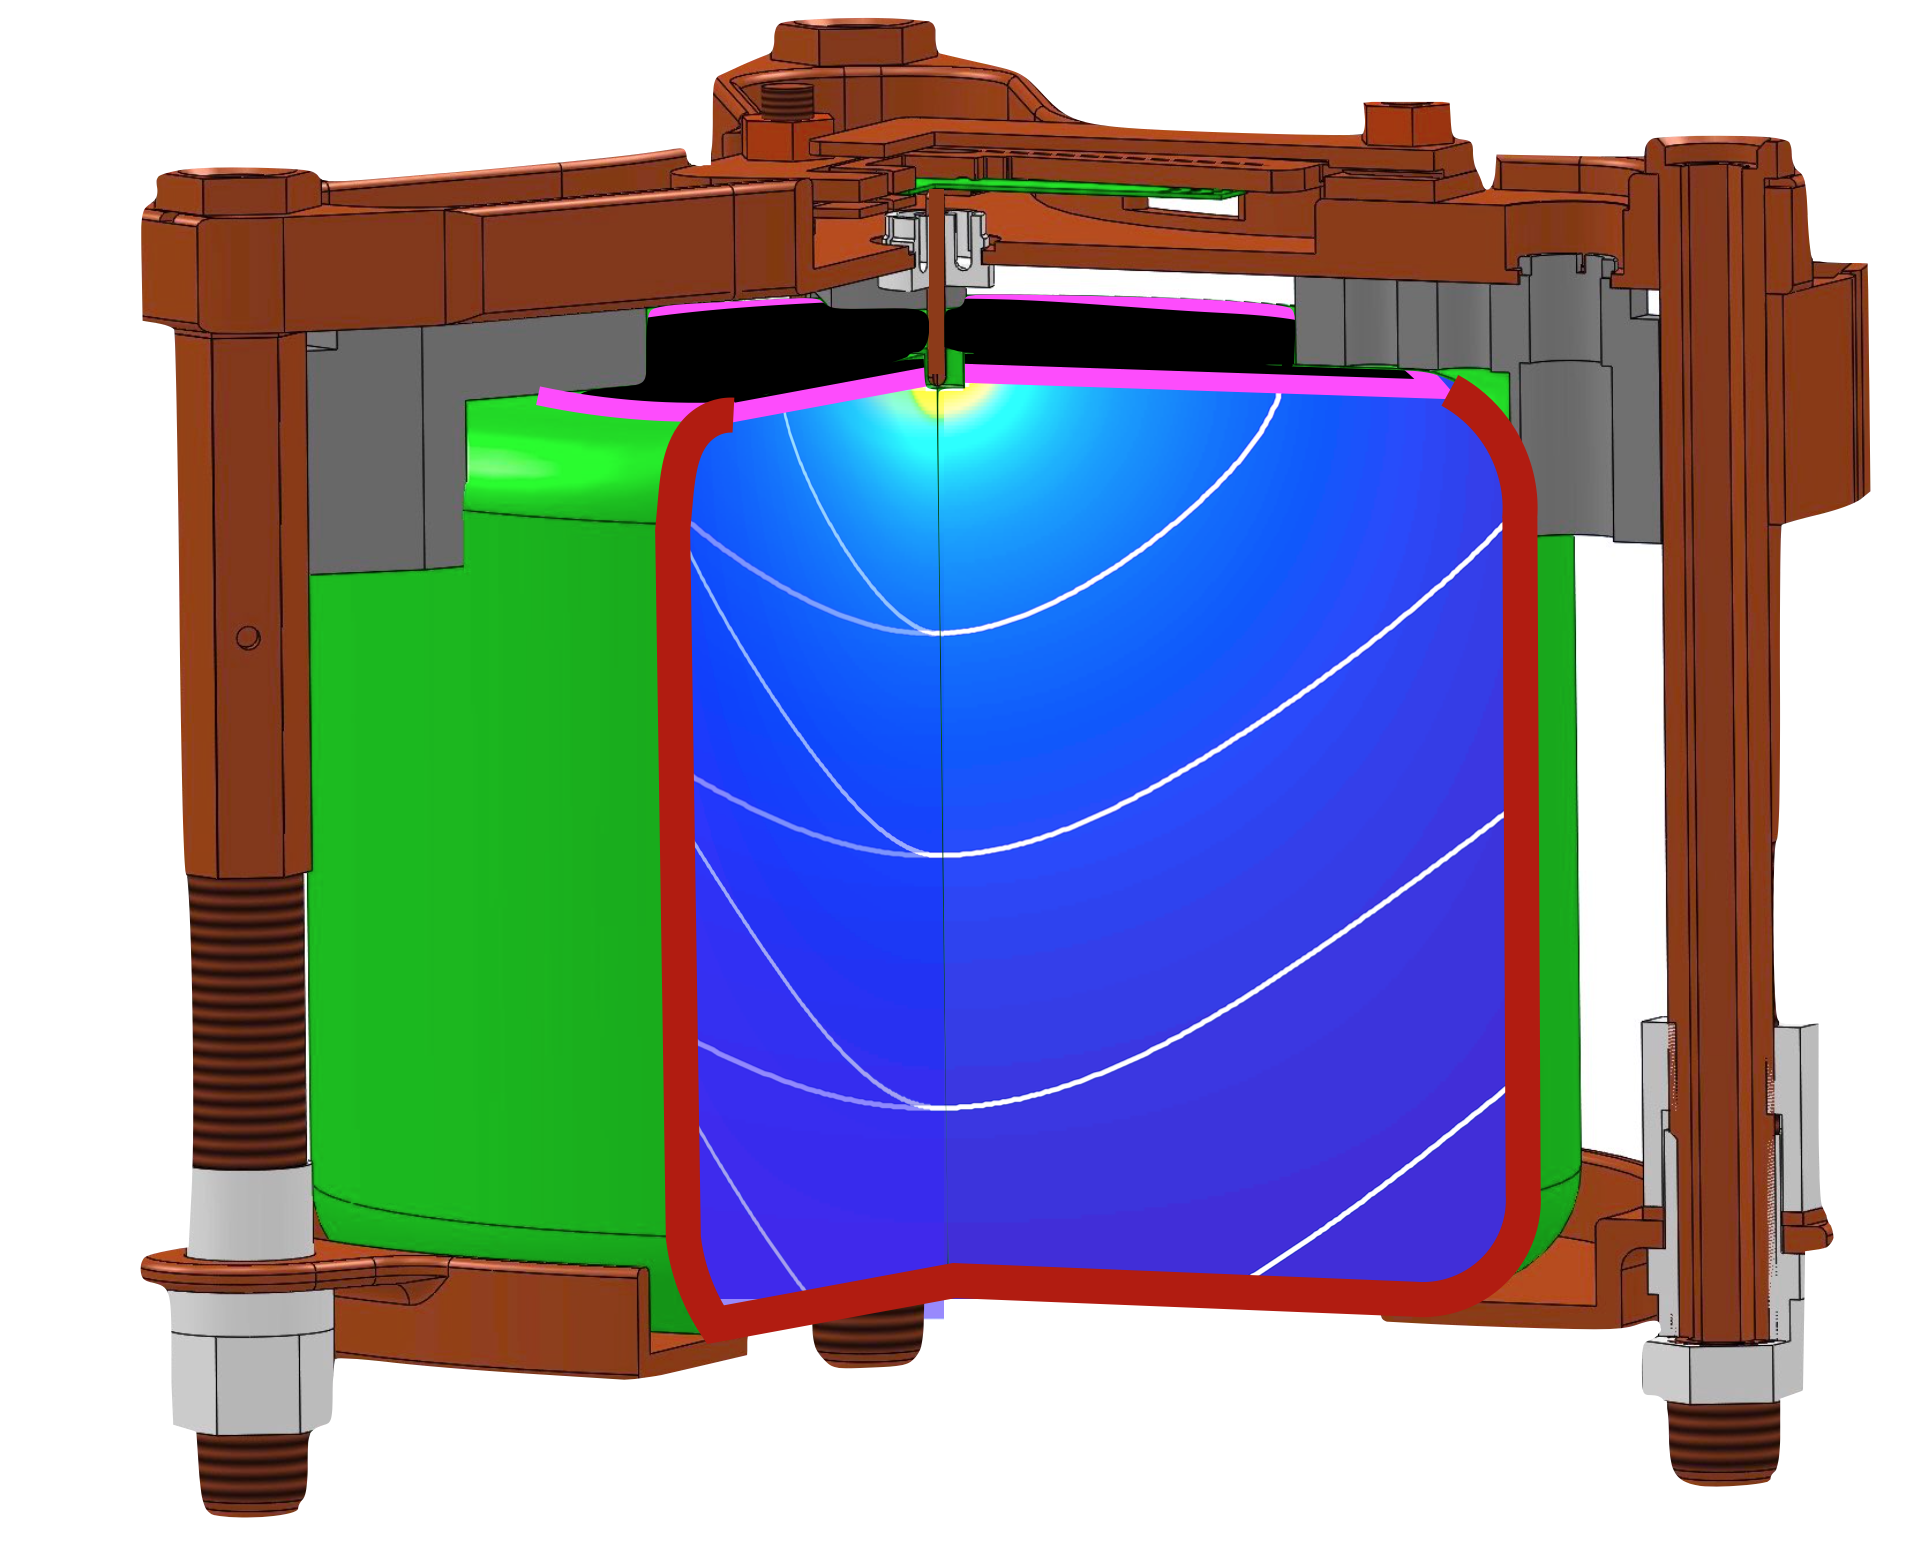
\includegraphics[width=0.8\columnwidth]{ppc_surfaces.png}
        \caption{Illustration of ``OPPI-1'', a PPC HPGe detector in a \MJ-style holder.
        The passivated surface ($\mu$m-thick) is shown in black.
        The outer Ge(Li) n$^+$ contact (green) is shown with its mm-thick transition region (red), and the boundary with the passivated surface (magenta).
        Bias is applied through the lower surface, and signals are initially amplified by a front-end electronics board near the point contact.
        }
        \label{fig:surfaces}
    \end{figure}
    
    In contrast, ionization events near the p$^+$ contact (typically boron-doped), and the surface passivation layer separating the two contacts, have been less well-characterized and focused on $\alpha$-particle events.
    These $\alpha$ decays from isotopes including $^{210}$Po can deposit several MeV in the detector as their ionization tracks penetrate the thin amorphous layers~\cite{majorana2018, othman2021cage, gruszko2022alpha}.
    These events exhibit two notable features, a sharp rising edge as some holes are immediately collected at the p$^+$ contact, and a ``delayed charge collection'' component, as a slow surface current propagates along the passivated surface.
    Recent studies of the p$^+$ and passivated surface response have shown that low-energy photon events (typically $\gamma$-rays) also induce an $\alpha$-like signal with a fast rising edge~\cite{othman2021cage, cdex2022passivated}.
    However, the detector response to incident electrons (typically $\beta$'s) has not been directly measured. It is believed, given a constant dead region near the passivation surface, that low energy photons and electrons could experience energy degradation similar to that of $\mathcal{O}(5~\mathrm{MeV})$ alphas given their similar penetration depths in germanium (SHOW PENETRATION DEPTH PLOT WITH PHOTONS, ELECTRONS, ALPHAS?

    \begin{figure}
        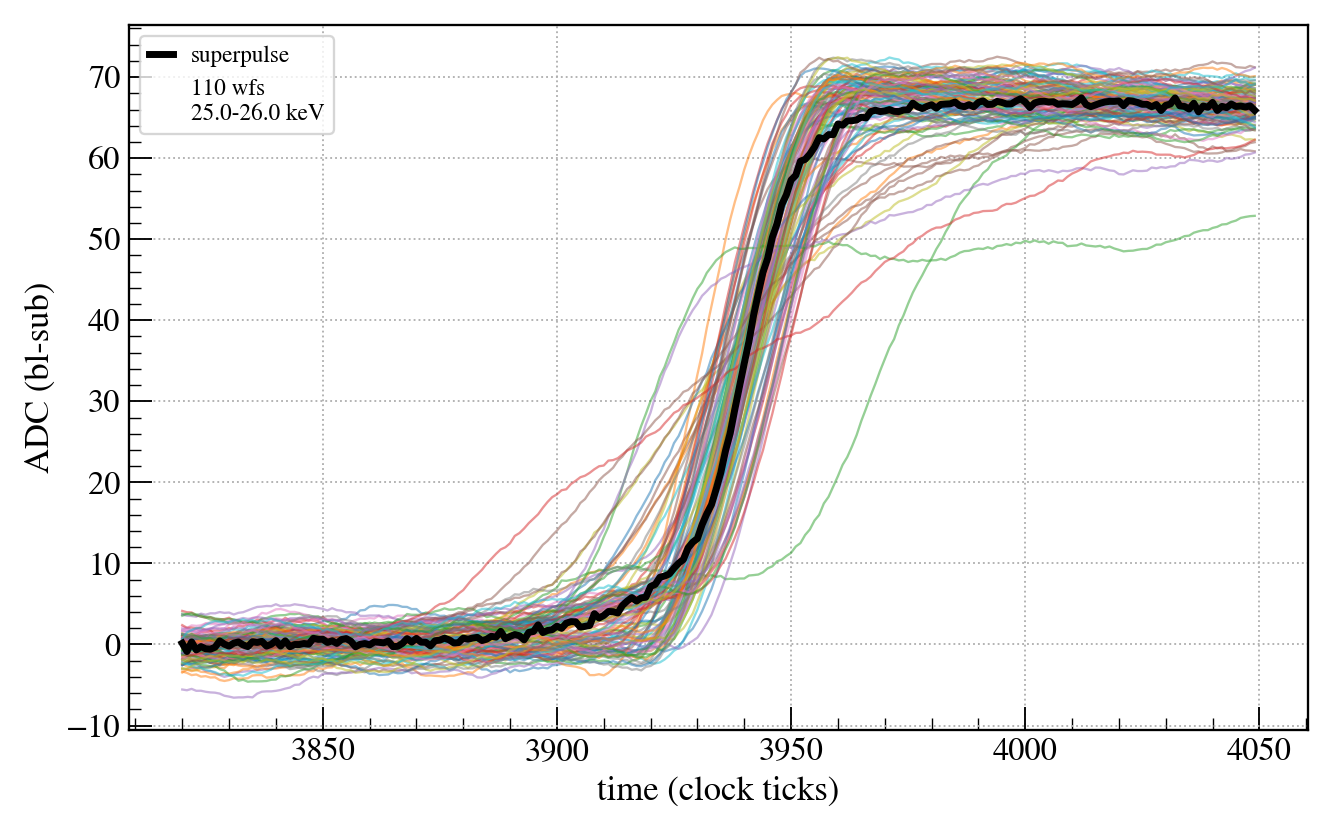
\includegraphics[width=\columnwidth]{krstc_waveforms.png}
        \caption{Placeholder. Average waveforms from the HPGe detector bulk from $\gamma$-rays (blue), and the \kr83 surface events (red).  What we want to show here is two superpulses, one of bulk signals, and one of \kr83 surface event signals with the obvious rise.  Probably we can use T/E or rise-time to select these signals.}
        \label{fig:waveforms}
    \end{figure}

    Using a \MJ\ PPC HPGe detector prototype, a vacuum cryostat, and an $^{83}$Rb source which produces gaseous metastable krypton (\kr83), we measured the detector response to monoenergetic low-energy electrons ($\sim30$ keV) and photons (9, 12 keV).
    The observed energy degradation from a single-energy electron signal allows a measurement of the passivated surface charge collection profile, and we show that the electron signals are also distinguishable from bulk events.
    In this work we describe the experimental setup, energy spectrum and pulse shape analysis of a series of Kr and background data collections, and compare to simulations to extract a model of the expected energy loss for passivated surface events, which in principle is generalizable to all HPGe detectors of similar design.

    % The low energy spectrum from the \MJD\ shows a rise in the \enrge\ detectors, whose surface exposure was stringently limited to reduce cosmogenic activation~\cite{wiseman2022exotic}, that may be explained by $\beta$ decays from $^{210}$Po and associated isotopes. % idk, this might just look like speculation until the exotic DM paper is published


\section{Experimental Setup}
    % slow controls, temp monitoring, etc.  systematics.

    We deployed a 0.5X~kg prototype PPC HPGe detector manufactured in 201X by ORTEC for \MJ\ in a liquid nitrogen (LN) vacuum cryostat originally designed for characterization of multi-detector strings.
    The detector is held in a Cu mount and surrounded by a thin-walled Cu infrared (IR) shield.
    Signals from the detector are read out at the front end near the point contact with a resistive feedback amplifier, using an XX-XXXX JFET and 10~G$\Omega$ feedback resistor, similar to Ref.~\cite{majorana2022electronics}.
    The first-stage waveforms have an RC decay constant $\tau_1 = 1.3$~ms, and are further amplified with a second-stage outside the cryostat, which removes a DC offset and shapes the signals with an RC decay $\tau_2 = 73\ \mu$s.
    The signals are saved as 80~$\mu$sec waveforms using a Struck 3302 digitizer at 100~MHz, using the ORCA data acquisition software~\cite{howe2008orca}.
    Fig.~\ref{fig:readout} shows a block diagram of the readout chain.

    \begin{figure}
        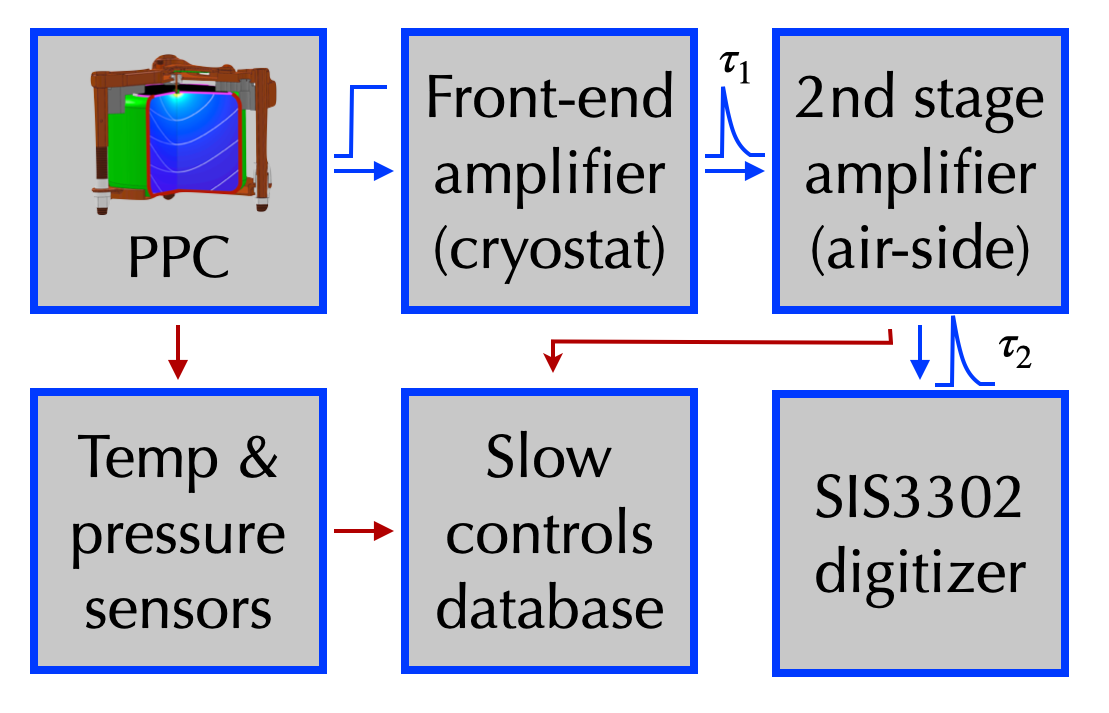
\includegraphics[width=\columnwidth]{krstc_readout.png}
        \caption{Block diagram of the DAQ and slow controls readout.  We may also need to create a vacuum valve diagram, might be able to squeeze it in here with a couple more boxes.}
        \label{fig:readout}
    \end{figure}    
    
    Slow controls data is saved using the Dripline framework~\cite{laroque2022dripline}, including the detector leakage current, pressure with a Pfeiffer PKR 251 vacuum gauge, and temperature with a thermally-lagged PT1000 sensor\footnote{TEWA TT4-PT1000B-T125-M5-500.   And maybe other part numbers listed down here?  RPi ADC chip too?} ARE WE SURE IT'S A PT1000??? calibrated to 77~K when direcly immersed in liquid nitrogen (WHEN DID THIS HAPPEN? GRACE AND I DIDN'T REALLY CHECK THIS) and mounted to the top of the Cu IR shield.
    The cryostat is pumped via a HiCube Eco 80 turbopump to vacuum levels of $10^{-6}$~mbar while warm, and when cooled with liquid nitrogen (LN) via a Cu cold finger, attains a minimum pressure $10^{-8}$~mbar due to cryopumping of residual gases on the cold surfaces.
    When the turbopump is valved off, the system maintains a $10^{-6}$~mbar vacuum purely from cryopumping, and the \kr83 source is valved in and allowed to outgas into the volume.

    \begin{table}
        \caption{Expected decay products from the \kr83 source~\cite{mccutchan_nuclear_2015}, with their expected attenuation lengths in germanium~\cite{nist_xcom, nist_estar}.  
        The mean free path of the low-energy \kr83 decay products is too short to penetrate the n$^+$ layer, confining the active region to the passivated surface.
        Between 30 and 17 keV, the signature is dominated by the monoenergetic $\sim$ 30 keV electrons. PLOT THE PENETRATION DEPTHS AS WELL? OR IS A TABLE SUFFICIENT?
        }
        \clearrow
        \begin{tabular}{>{\rowmac}l|>{\rowmac}c|>{\rowmac}c|>{\rowmac}c<{\clearrow}}
            \hline\hline
                 & Energy & Intensity  & Mean depth \\
                 & (keV)  & (\%)       & in Ge ($\mu$m) \\
            \hline\hline
            $\gamma$ & 32.15 & 0.1  & \\
            CE N & 32.12 & 0.8  &  \\
            \setrow{\bfseries} CE M & 31.86 & 10.7 &  \\
            \setrow{\bfseries} CE L & 30.23 & 63.7 & \\
            \setrow{\bfseries} CE K & 17.82 & 24.8  &  \\
            XR $k_{\beta 1}$ & 14.31 & 0.2 & \\
            XR $k_{\beta 2}$ & 14.11 & 1.3 &  \\
            XR $k_{\beta 3}$ & 14.10 & 0.7 & \\
            \setrow{\bfseries} XR $k_{\alpha 1}$ & 12.65 & 9.1 & \\
            XR $k_{\alpha 2}$ & 12.60 & 4.7 & \\
            Auger K & 10.80 & 8.6  &  \\
            $\gamma$ & 9.41 & 5.5 &  \\
            CE N & 9.38 & 1.3 &  \\
            \setrow{\bfseries} CE M & 9.11 & 12.9 & \\
            \setrow{\bfseries} CE L & 7.48 & 80.0 &  \\
            % XR l & 1.59 & 3.7  &  \\ % below detection threshold of 5 keV
            % Auger L & 1.5 & 168.4 & 1 mm \\
            \hline\hline
        \end{tabular}
        \label{tab:signals}
    \end{table}
    
    Several similar \kr83 sources have been produced by PNNL for the KATRIN~\cite{venos2018properties}, Project 8~\cite{project8cres2015}, and He6-CRES~\cite{he6cres2022} experiments, all making use of the monoenergetic 30~keV electron signal.
    A $^{83}$Rb parent is embedded in a microporous zeolite, and contained in a stainless-steel capsule containing multiple filter layers such that the only products allowed to escape are gaseous, including nitrogen, argon, and krypton.
    The $^{83}$Rb decays to \kr83, which has a 1.83~hour half-life (CITE NUDAT???).
    This is long enough for the krypton to diffuse out of the source by Brownian motion.  
    A small fraction of \kr83 is able to penetrate a small opening in the top of the IR shield and fill the volume above the detector passivated surface before decaying.
    Table~\ref{tab:signals} gives a full list of decay products observable above a 5~keV threshold, including their expected penetration depths in pure Ge.
    The rate of Kr outgassing from $^{83}$Rb is not measured directly, but the rate is low enough for the cryopumping to maintain a vacuum level of $10^{-6}$~mbar when the source is valved in.

    \begin{table*}[ht]
        \caption{Data taking campaigns with the \kr83 source, alternating Kr and background runs.  
        Mean detector temperature and pressures are reported, with typical daily variations on the order of 1 K and $1 \times 10^{-9}$ mbar, respectively.}
        \begin{tabular}{ccccccl}
            \hline\hline
                     &      & Run   & Run time & Detector & Presssure &  \\
            Campaign & Date & Type  & (hrs)    & temp (K) & (mbar)         & Notes \\
            \hline\hline
            % note: don't change the numbering of the campaigns in the elog.  we'll just start w/ later numbering here, starting with Campaign 6.
            6 & 2/15/2023 & Bkg & 15 hrs & 88.1 & $1 \times 10^{-6}$ & thermally-lagged temp sensor (i thought we had this from C9?) \\
            6 & 2/16/2023 & Kr & 16 hrs & 88.2 & $1 \times 10^{-6}$ & \\
            6 & 2/17/2023 & Kr Decay/Bkg & 21 hrs & 88.2 & $1 \times 10^{-6}$ & thermally-lagged temp sensor \\
            6 & 2/18/2023 & $^{133}$Ba & 0.2 hrs & 88.2 & $1 \times 10^{-6}$ & thermally-lagged temp sensor \\
            6 & 2/18/2023 & pulser & 5 hrs & 88.1 & $1 \times 10^{-6}$ & following bake to 50 C for 12 hr, 1 10dB/50$\Omega$ attenuator \\
            6 & 2/18/2023 & pulser & 5 hrs & 88.1 & $1 \times 10^{-6}$ & 3 10dB/50$\Omega$ attenuators\\
            % 8 ...
            % 9 ...
            9 & 4/21/2023 & Bkg & 1 hrs & 87.7 & $1.9\times 10^{-7}$ & Found a slow leak, this pressure is before closing the valve, and det depleted at 2200V \\
            9 & 4/21/2023 & Kr & 18 hrs & 87.7 & $1.9\times 10^{-7}$ & Found a slow leak, raised threshold to 0x9 for 3061 \\
            9 & 4/22/2023 &  & 18 hrs & 87.7 & $1.9\times 10^{-7}$ & Found a slow leak, raised threshold to 0x9 for 3061 \\
            \hline\hline
        \end{tabular}
        \label{tab:campaigns}
    \end{table*}
    
    The potential adhesion of the krypton gas to the cold detector is strongly dependent on the temperature of the surface, the surface itself, and the vapor pressure of krypton at low temperatures.
    Nominally krypton is able to freeze at temperatures lower than 120 K, but in practice a lower temperature is desirable to increase the probability.
    Using indium wire to increase the thermal conductivity of the various pieces of the Cu cold finger assembly, our system has achieved temperatures as low as 88~K.
    Some uncertainty in the true temperature exists due to the use of a single PT1000 (???) sensor on the top of the IR shield; we take a 10\% systematic uncertainty to be conservative.
    The cryostat is equipped with a set of cartridge heaters on the LN dewar, allowing an accelerated warmup cycle, and the capability to bake to $\sim$60~C to remove water vapor.     
    % As we will show in Sec.~\ref{sec:analysis}, the shape and amount of energy degradation of the observed \kr83 spectrum is highly correlated with temperature and the amount of water vapor deposited on the detector surface from exposure to room air during installation.
    As we will show in Sec.~\ref{sec:analysis}, the shape and amount of energy degradation of the observed \kr83 spectrum is highly correlated with the pressure of the cryostat at the start of the liquid nitrogen cool down process. It is thought that when cooling down at higher pressures ($\mathcal{O}(4 \times 10^{-6}~\mathrm{mbar})$) there is more water vapor and other residual gas in the cryostat which then condenses on the passivated surface and changes detector performance. The krypton is not thought to stick stronly to the germanium as the krypton rate rapidly decreases when valving in the vacuum pump to the system.

    Several multi-day data taking campaigns were conducted at various temperatures and operating voltages, described in Table~\ref{tab:campaigns}.
    These campaigns were partitioned into background data taking periods where the turbopump was valved in and out, \kr83 runs where the source was opened with the turbopump valved out, and various calibration cycles including electronic pulser scans and $^{133}$Ba low-energy calibrations. Decay runs were also taken, transitioning from krypton runs to background runs as the krypton decayed away with the expected half-life. 

    

\section{Analysis} \label{sec:analysis}
    % main selling points: characteristic energy spectrum and waveform shapes.  
    % - could potentially break this into subsections, if it goes longer than ~2 pages.

\subsection{Energy Spectrum}

    The primary goal of this study was to exploit the electron signal at $\sim$30 keV to extract information about the energy degradation of electron events at the passivated surface, since the signal is monoenergetic as opposed to a $\beta$-decay continuum.
    The strength and shape of the \kr83 signal was observed to vary significantly with the condition of the detector surface.
    The strongest spectrum observed was in Campaign 9 after initial receipt of the source, and is shown against its corresponding background data set in Fig.~\ref{fig:spectrum}. OR SHOULD WE JUST SHOW SOME COMBINED SPECTRUM? WE'LL SEE WHAT LOOKS GOOD. 
    Several features from Table~\ref{tab:signals} are evident in the spectrum.
    No peak exists at 30~keV, indicating that all electron signals are at least partially energy-degraded. Energy degradation of the highest energy electrons is roughly linear in some runs (C9) and more ``shelf-like'' (NEED BETTER TERMINOLOGY) in others with different detector conditions. 
    An upturn starting at $\sim$17~keV indicates the presence of more conversion electrons, and notably, two photon lines are observed at 12.6~keV, and 9.4~keV.
    The X-ray line at 12.6~keV shows that the \kr83 undergoes atomic excitation and deexcitation as part of the decay to stable Kr.

    \begin{figure}
        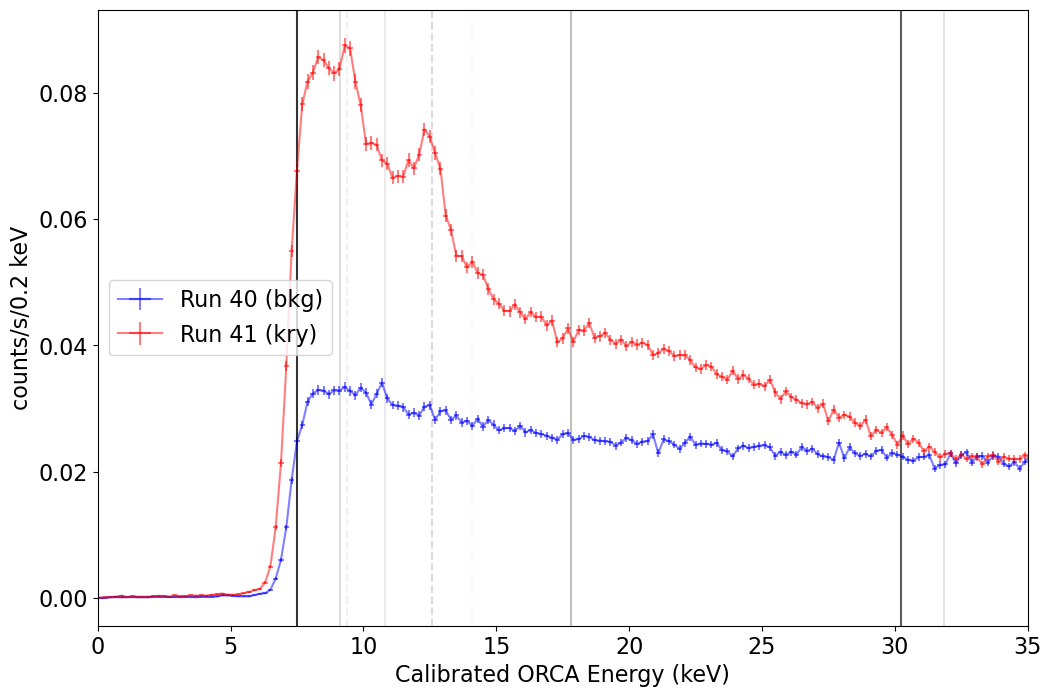
\includegraphics[width=\columnwidth]{krstc_spectrum.png}
        \caption{\kr83 signal vs background.  Solid lines indicate monoenergetic electron signals, dashed lines are photon signals.  An X-ray at 12.6~keV is observed, along with a gamma at 9.4~keV.}
        \label{fig:spectrum}
    \end{figure}
    
    Since the presumed dead layer near the passivated surface is only $\mathcal{O}(\mu$m)-thick, monolayers of water vapor or other gases can have a significant effect.
    Additionally, the outgassing rate of the zeolite can vary over time as impurities from other gases clog the micropores of the zeolite, preventing Kr from outgassing. 
    Significant effort was undertaken to reproduce the initial strong signal from Campaign 6, including a pump-and-bake cycle of the $^{83}$Rb source and the detector.
    The variation in the energy spectrum for different detector behaviors is given in Fig.~\ref{fig:variation}.
    
    \begin{figure}
        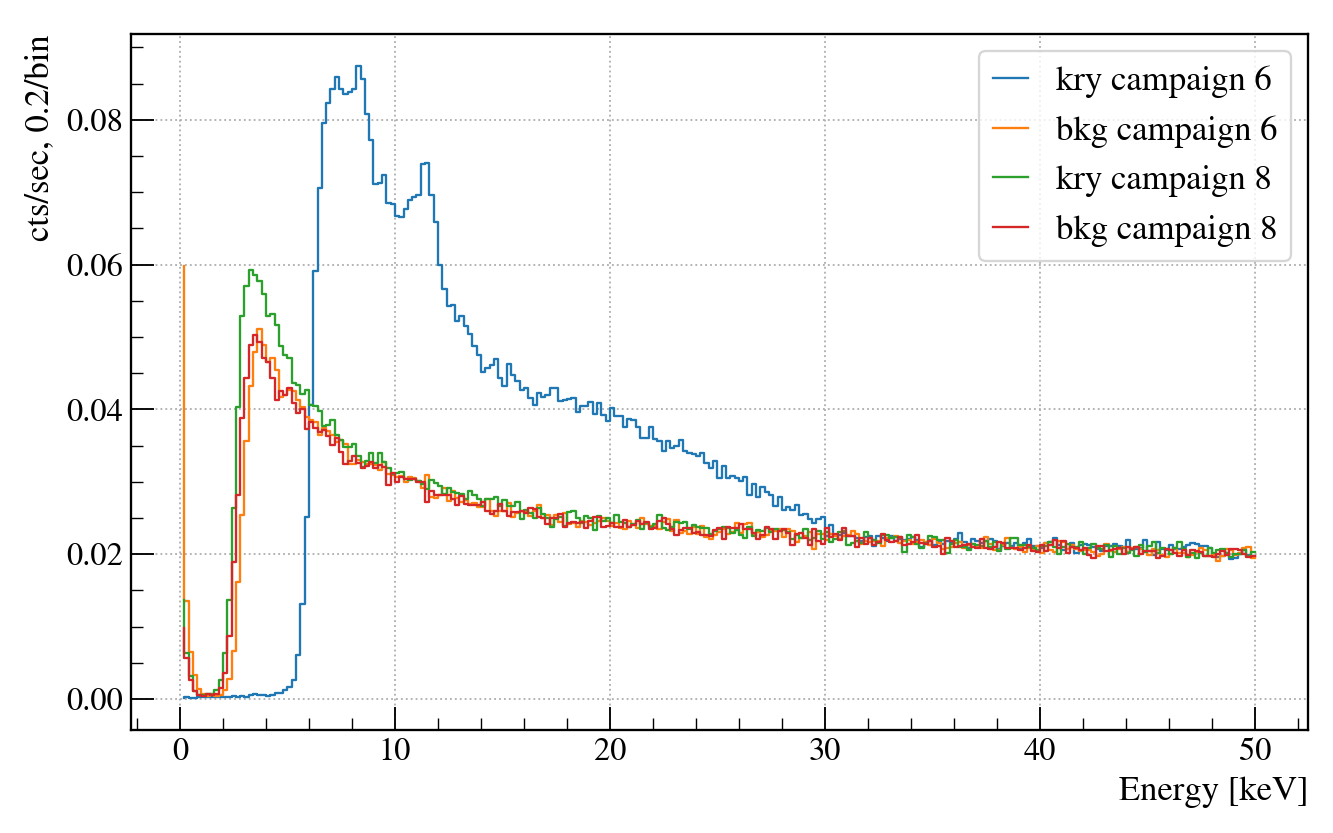
\includegraphics[width=\columnwidth]{krstc_spectrum_variation.png}
        \caption{Placeholder: show a figure with the variation in the Kr spectrum, after various pumps/bakes/cooldowns etc.}
        \label{fig:variation}
    \end{figure}

\subsection{Waveform Analysis}
    % Show a T/E vs E or risetime plot - whatever we end up using to pick out the surface event signals.  

    Previous studies from \MJ, TUBE, CAGE, and CDEX strongly suggested that an observable difference in the pulse shape may exist for near-passivated surface events.
    The difference between the surface event and bulk waveforms allows various pulse shape analysis (PSA) parameters to be employed.
    As illustrated in Fig.~\ref{fig:waveforms}, waveforms from the \kr83 surface events show evidence of a fast-rising component. This is to be expected, as rapid charge collection occurs as holes drift near the p+ point contact.
    Two techniques were employed to identify surface events, one based on the rise time to 20\% of the full amplitude, and another using a short trapezoidal filter with no gap time (triangle filter)~\cite{knoll2010radiation}.
    Both methods are conceptually similar to taking a derivative of the voltage signal.   
    
    The rise time method is in principle more sensitive to the sharp change at the beginning of the pulse, but due to the relatively low signal-to-noise ratio at keV-scale energies, is susceptible to false positives if a smoothing function is not applied to the waveform.
    % We select a Savitzky-Golay filter from \texttt{scipy}, \texttt{savgol_filter}~\cite{scipy2020}, with coefficients (XX, XX, XX).
    % Fig.~\ref{fig:risetime} shows the distribution of rise times scaled by energy.

    \begin{figure}
        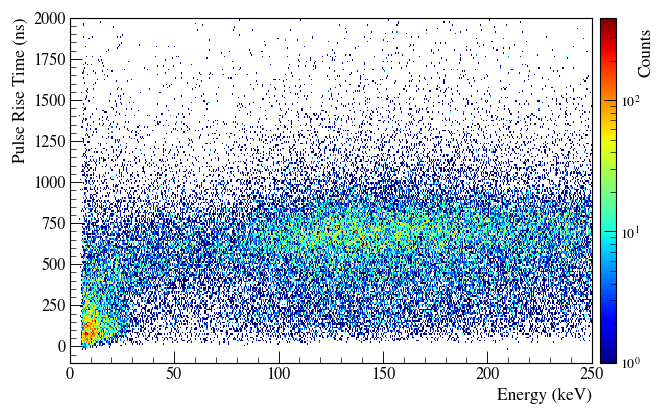
\includegraphics[width=\columnwidth]{risetimes.png}
        \caption{Placeholder for 2d risetime vs energy figure.}
        \label{fig:risetimes}
    \end{figure}
    
    \begin{figure}
        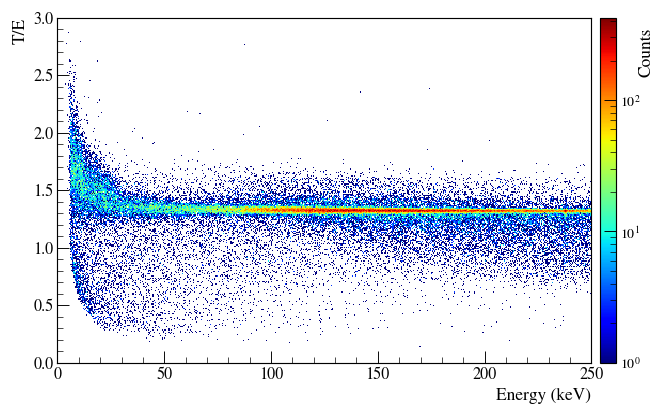
\includegraphics[width=\columnwidth]{trianglefilt.png}
        \caption{Placeholder for 2d T/E vs E figure.}
        \label{fig:toe}
    \end{figure}
    
    The longer integration time of the triangle filter allows some smoothing of


\section{Simulation of Surface Events}
    % simple model of passivated layer, surface charge
    \subsection{Krypton Decay Simulation}
    % Simulated Kr decays with Josh's code, considered energy threshold, detector resolution, n+ dead layer.
    Performing a simulation of these surface krypton events is crucial to understanding the nature of the energy degradation and uncovering the detector dead layer. \kr83 undergoes a two-level decay from a second excited energy state at 41.6 keV to a first excited state at 9.4 keV to the stable ${}^{83}$Kr ground state. This can produce a number of ejecta as shown in Table~\ref{tab:signals} with coincident products from the second and first excited state separated in time by 156 ns on average. Code was produced to generate individual \kr83 decays from the energies and intensities given in~\cite{mccutchan_nuclear_2015}. These decay products were then given some random initial position inside the detector's IR shield and each ejecta received some random momenta assuming an isotropic distribution for all decay products. DID I CHECK IF THEY WENT THROUGH THE PASSIVATED SURFACE? The generated decays were collated and put through an edited version of g4simple (CITE?) and simulated with the ``Shielding'' physics list in GEANT4 (CITE?). 

    The resulting spectrum from 5 million simulated Kr decays is shown in Fig.~\ref{fig:sim_spectrum}. From the simulated spectrum we can apply an estimated energy threshold, a millimeter-thick n+ dead layer, and an energy resolution function taken from data. There are clear peaks at all energies of higher intensity electron and photon lines as well as peaks corresponding to summed coincident 32.1 keV and 9.4 keV decays. 

    \begin{figure}
        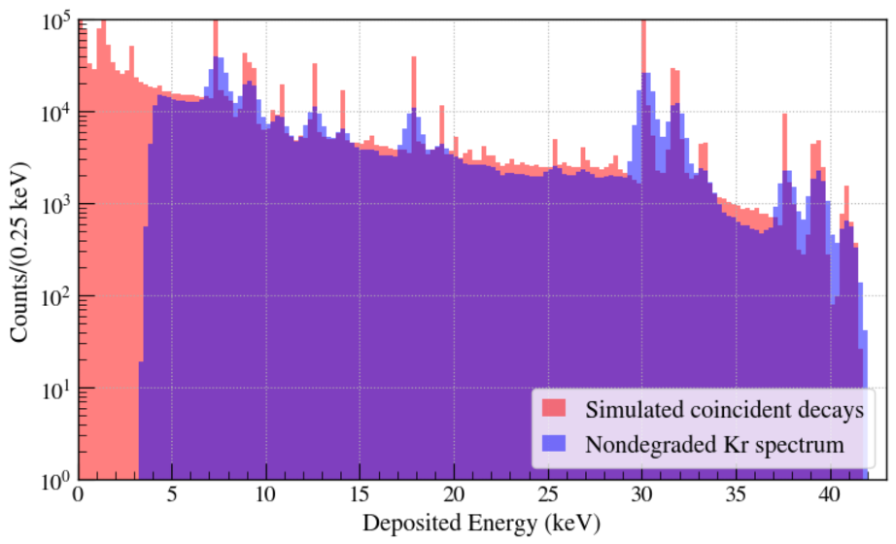
\includegraphics[width=\columnwidth]{figures/simulated_Kr_spectrum.png}
        \caption{Placeholder: $^{83m}$Kr spectrum as seen by OPPI, simulated using Geant4 (g4simple?). Post-processed spectrum considers energy threshold, detector resolution, and n+ dead layer. GET RID OF ``COINCIDENT,'' IT'S CONFUSING. Also maybe remake spectrum without the fill?}
        \label{fig:sim_spectrum}
    \end{figure}

    \subsection{Simulated Surface Charge and Ge Pulses}
    % Using siggen, simulated many different surface charges. Stopped collecting charge carriers after drifted to PS. Found activeness map for surface charges (elephant ears) and applied those to simulated spectra to match data. Also found theta dependence. Also also looked into diffusion (more important) and self-repulsion (less important). 
    If surface charges are indeed a component of the energy degradation seen in KrSTC then a Ge waveform simulation is of clear importance. We utilized the Ge charge carrier simulation package \texttt{siggen}~\cite{radford2022siggen} to generate energy depositions near the detector passivated surface and study the effect that surface charges on that surface has on charge collection. 

    \subsubsection{Surface Charge Induced Dead Layer}

        The proposed physical mechanism (we think this because of CITE SOMETHING?) by which surface charges induce a dead layer is as follows: if we apply a uniform negative (positive) static charge to the passivated surface, as holes (electrons) drift near that surface, they will experience an attractive force and drift towards the surface charge. That charge then gets trapped and released on a time scale longer than is visible to us and thus is modeled as a stop in charge collection once a charge carrier reaches the passivated surface. Due to the ``hole-dominated'' nature of the waveforms (as governed by the large weighting potential near the p+ point contact, WEIGHTING POTENTIAL PLOT? MENTION SHOCKLEY-RAMO?), a negative surface charge would create a significantly larger dead layer than a positive one. This study primarily considers negative surface charges to more closely recreate the significant energy degradation we see in data.

        We generated a grid of ($\sim100k$???) single site energy depositions distributed linearly across all radial detector coordinates and logarithmically spaced axially, from $1~\mu$m to $50$~mm. The induced charge from drifting charge carriers that have reached the passivated surface were not considered, leading to a map of fractional charge collection for various surface charge configurations. This map was then applied to the GEANT4 simulations to produce an expected spectrum. One such activeness map and resulting spectrum are shown in Fig.~\ref{fig:minus3e9_sim_spectrum}. This activeness map considers only energy depositions at an azimuthal cylindrical angle $\varphi = 0$~rad. The effect of this angle is discussed later, in Section ????

            % Stacking images not working

% \begin{figure}
%   \centering
%   \begin{tabular}{@{}c@{}}
%     \includegraphics[width=.7\linewidth,height=75pt]{example-image-a} \\[\abovecaptionskip]
%     \small (a) An image
%   \end{tabular}

%   \vspace{\floatsep}

%   \begin{tabular}{@{}c@{}}
%     \includegraphics[width=.6\linewidth,height=100pt]{example-image-b} \\[\abovecaptionskip]
%     \small (b) Another image
%   \end{tabular}

%   \caption{This is a figure caption}\label{fig:myfig}
% \end{figure}

    \begin{figure}
        \begin{tabular}{@{}c@{}}
            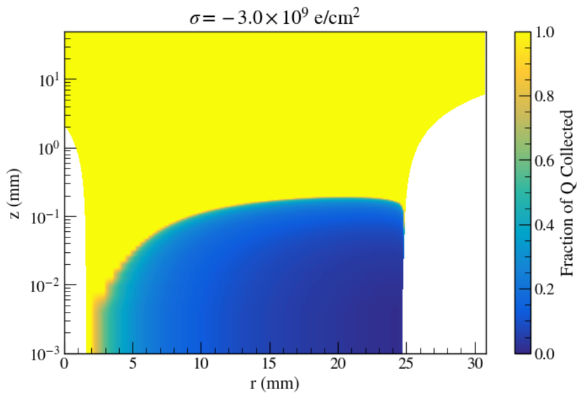
\includegraphics[width=\columnwidth]{figures/minus3e9_activeness_map_theta0.png} \\[\abovecaptionskip]
            \small (a)
        \end{tabular}
        
        \vspace{\floatsep}
        
        \begin{tabular}{@{}c@{}}
            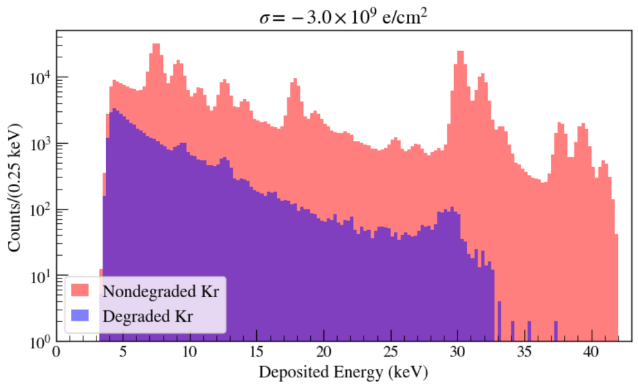
\includegraphics[width=\columnwidth]{figures/minus3e9_simulated_Kr_spectrum.png} \\[\abovecaptionskip]
            \small (b)
        \end{tabular}
        
        \caption{Placeholder: (a) Activeness map with an applied surface charge density of $\sigma = -3 \times 10^{9}$ e/cm$^2$ and fixed azimuthal angle $\varphi = 0$~rad, simulated with siggen. (b) That activeness map applied to the simulated spectrum from \ref{fig:sim_spectrum}.}
        \label{fig:minus3e9_sim_spectrum}
    \end{figure}

    % \begin{figure}
    %     \begin{subfigure}
    %         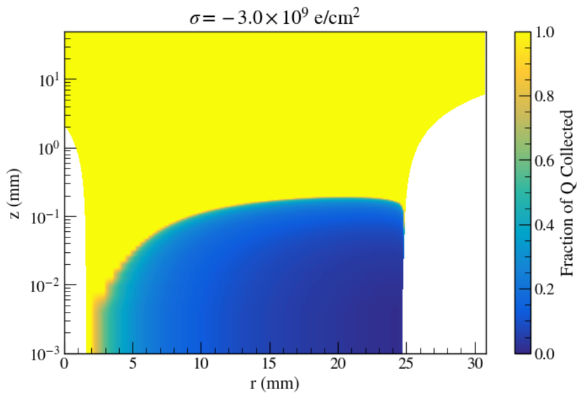
\includegraphics[width=\columnwidth]{figures/minus3e9_activeness_map_theta0.png}
    %         \caption{}
    %         \label{fig:minus3e9_activeness}
    %     \end{subfigure}
    %     \vfill
    %     \begin{subfigure}
    %         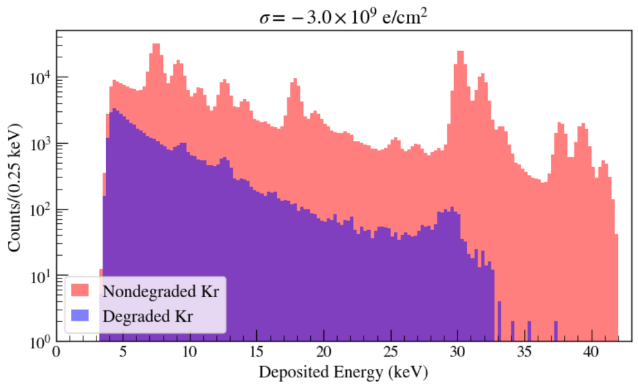
\includegraphics[width=\columnwidth]{figures/minus3e9_simulated_Kr_spectrum.png}
    %         \caption{}
    %         \label{fig:minus3e9_sim_spectrum}
    %     \end{subfigure}
        
    %     \caption{Placeholder: (a) Activeness map with an applied surface charge density of $\sigma = -3 \times 10^{9}$ e/cm$^2$, simulated with siggen. (b) That activeness map applied to the simulated spectrum from \ref{fig:sim_spectrum}.}
    % \end{figure}

        A surface charge density of $\sigma = -3.0 \times 10^9$~e/cm$^2$ produces a layer that extends past $z = 100$~$\mu$m into the detector. This dead layer is large enough to degrade the energies of all electrons in this energy range and some photons as well. This follows what data shows us, with all electron lines fully suppressed and some photon line component visible in the energy spectrum. There are still unresolved issues, however, particularly regarding the energy degradation of the L-shell conversion electron (CE L) with energy $E = 30.23$~keV and intensity $I = 63.7\%$. The $18~\mathrm{keV} < E < 30$~keV region of the spectrum is useful to study due to this dominant electron line (and subdominant $E = 31.86$~keV CE M line) with no other decay products between it and the K-shell conversion electron at $E = 17.83$~keV. It appears in data that the energy degradation is approximately linear in this region in some runs and more ``shelf-y'' (HOW DO I SAY THIS) in others with different run conditions. 

        Also talk about how photon peaks shrink but are still there, electrons are all degraded. Negative surface charge almost consistent-ish with our data, but that means there's way more negative surface charge when the detector is clean which you'd expect to affect detector performance (biasing, depletion, etc.) more. Say something about the stuff getting on the surface and reducing the magnitude of the surface charge. 


    \subsubsection{Theta Dependence}

    Another consideration regarding the surface charge-induced dead layer is the azimuthal angle in the detector at which a charge carrier is drifting. It is known (CITE papers from Ben Shanks) that the drift velocity of the charge carriers is not necessarily parallel to the direction of the electric field. This is due to mobility differences--in both holes and electrons--along the different FCC crystal axes of the germanium. These axes are not orthogonal to each other but the true drift velocity can be calculated (DON'T LIKE THIS SENTENCE!). 

    THINKING MAYBE WE SHOULD HAVE ANGLE DEPENDENCE BEFORE SHOWING THE ACTIVENESS MAP AND SPECTRUM BC WE WANT TO INCLUDE THETA IN THE MODEL.

    This angle dependence will affect the size of the dead layer at the $\mathcal{O}(10\%)$ level, as shown in Fig.~\ref{fig:contours}.
    
    \begin{figure}
        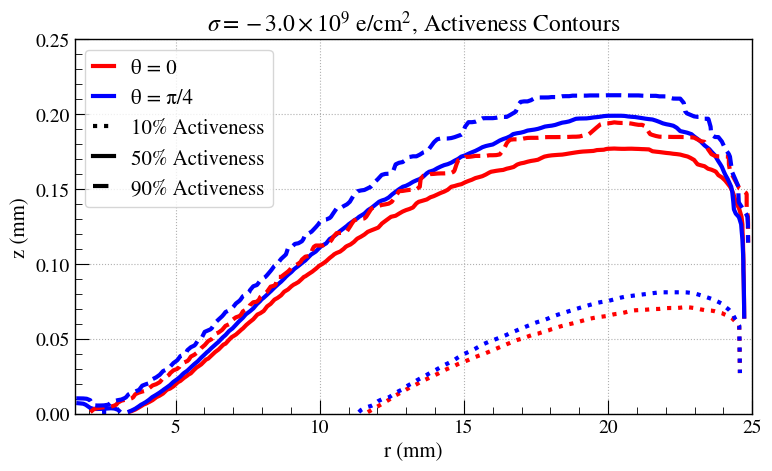
\includegraphics[width=\columnwidth]{figures/minus3e9_contours_thetastudy.png}
        \caption{Placeholder: Theta dependence of different activeness contour lines for a $\sigma = -3 \times 10^{9}$ e/cm$^2$ charge density. Effect is symmetric about $\theta = \pi/4$.}
        \label{fig:contours}
    \end{figure}

    SHOULD WE SHOW ANOTHER ANGLE DEPENDENCE PLOT? LIKE PHI VS PSI OR JUST SHOW THE MOBILITIES?

    

    % A simple Geant4 model of the detector geometry was developed in conjuction with the Ge charge carrier simulation package \texttt{siggen}~\cite{radford2022siggen}, to simulate the \kr83 decay products and estimate the properties of the energy-degrading layer at the passivated surface.

    % \begin{figure}
    %     \includegraphics[width=\columnwidth]{elephant_ears.png}
    %     \caption{Placeholder: "elephant-ears" plot for PS degradation from varying levels of surface charge}
    % \end{figure}

    % \begin{figure}
    %     \includegraphics[width=\columnwidth]{sim-spectrum.png}
    %     \caption{Comparison of the observed \kr83 data spectrum with 2-3 simple models of PS deadness profile.}
    % \end{figure}
    

\section{Discussion}
    % application to LEGEND

    The observed variation in the \kr83 energy spectrum with surface effects makes an unambiguous measurement of the passivated layer energy-loss properties difficult with the current method.
    An absolute measurement of the detection efficiency is also not possible, since the fraction of Kr which cryopumps onto the detector surface versus the other cold Cu surfaces is not known.

    Other sources are in development for installation in the vacuum cryostat, including tuning the size of the dead layer using an electrode above the detector, and installing an X-ray fluorescence source which will send collimated photons at discrete energies into the passivated surface of the detector~\cite{elliott2023xrf}.
    However, the finding that the electron surface events possess the same characteristic rising edge as $\alpha$ and photon events is strong evidence that a pulse-shape analysis cut will be possible for the next generation of large germanium experiments.


\begin{acknowledgments}
    % need to check these with Jason & Walter

    We are grateful for many productive discussions with Alejandro Garcia, Drew Byron, Brent VanDevender, Steve Elliott, David Radford, and the engineering support at CENPA including David Peterson, Tim Van Wechel, Ryan Roehnelt, Nate Miedema, Matt Kallander, and Tom Burritt. 
    This material is based upon work supported by the U.S.~Department of Energy, Office of Science, Office of Nuclear Physics under contract / award number DE-AC02-05CH11231.  % need Jason and Walter's grant numbers
    % We gratefully acknowledge the support of the U.S.~Department of Energy through the Los Alamos National Laboratory LDRD Program and through the Pacific Northwest National Laboratory LDRD Program for this work.  
    This research used resources provided by the the National Energy Research Scientific Computing Center, a U.S.~Department of Energy Office of Science User Facility.

\end{acknowledgments}

\appendix

\section{Ideas for appendices}

A few nitty-gritty things we might want to include.  
Philosophy should be to make this paper self-contained, at least in the first draft.  
No damn unidocs for small group studies like this one!

\begin{enumerate}
    \item Slow controls vs Ge data cross-checks
    \item Energy resolution \& gain stability
    \item Calibration, noise performance
    \item Systematic studies (hardware changes)
\end{enumerate}



\appendix
\section{Shelf-like behavior tests}


\bibliographystyle{iopart-num}
\bibliography{krstc_refs}
\end{document}

    